\chapter{绪论}
%
\section{研究背景和意义}
%
在过去的二十年中,在机器人和航空领域,小型无人机(UAV)备受关注。 2010年以前,研究人员们主要关注无人机的控制算法\cite{Bouabdallah_2004,Castillo_2004}。 2010年之后,研究热点逐渐转移到无人机的多机编队\cite{Dong_2016,Wang_2012}或视觉导航\cite{Krajnik_2012,Lee_2012}上。 在最近五年中,消费级无人机市场已日渐成熟,以大疆为代表的无人机公司推出的四旋翼无人机备受青睐。 目前,许多无人机公司致力于将无人机应用到农业植保、快递运输、灾难救援、测绘、电力巡检等领域中。四旋翼无人机取得的成功标志着低成本、安全可靠的导航控制技术日渐成熟。

除四旋翼无人机外,针对特殊用途而设计的无人机也逐渐成为研究热点,例如垂直起见固定翼无人机\cite{Roberts_2010}、双旋翼无人机\cite{Siddhardha_2018}以及六自由度空中机器人\cite{Kamel_2018,Scholz_2016}等。

正是在无人机行业蓬勃发展的背景下,本文的研究了一类新型无人机——涵道风扇式无人机(Ducted Fan UAV,DFUAV)。DFUAV是一种垂直起降无人机,既可以高速盘旋又能在空中悬停。相比于固定翼无人机,DFUAV可用于海上平台等起飞空间狭小的环境中,还可以在复杂的城市环境或者丛林环境执行监控、检测等任务。与常规的直升机相比,在相同条件下涵道风扇可以产生更大的升力,并且可以获得更高的前飞速度。DFUAV结构紧凑,其风扇置于涵道内部,叶片受到涵道的保护,因而更适合在危险的环境中操作。DFUAV因其良好的实用性和广阔的应用前景,逐渐引起各国研究机构的重视。目前已有许多机型投入使用,如iSTAR\cite{Lipera_2001}、HoverEye\cite{Binetti_2007}等。

与传统的无人机相比,DFUAV气动布局独特,在垂直起降和前飞两种飞行模式下具有完全不同的气动特性\cite{Johnson_2005},因而其飞控系统设计极具挑战。在悬停时,进入涵道的气流保持对称,涵道周围产生的升力能保持平衡,涵道迎风与下风侧唇口产生的升力相等。当涵道以小攻角低速倾斜飞行时,此时流入涵道的气流不再对称,涵道周围产生的升力也不再对称\cite{Fleming_2004}。不对称气流在涵道上产生复杂的气动力矩,同时也使涵道底部的操纵面的升力系数发生变化,进一步增加控制系统设计的难度。

对全状态系统而言,DFUAV是一个欠驱动系统,其姿态跟踪性能直接影响速度跟踪性能。因此,姿态控制是DFUAV飞行控制系统的关键一环。在悬停飞行模式下,DFUAV的姿态受扰动影响较大,且通道之间的耦合比较严重。另一方面,本文研究的DFUAV其操纵面是冗余配置的,其姿态子系统是过驱动系统,存在控制分配问题。因此,研究DFUAV的控制分配问题及其与姿态控制器的结合,对解决DFUAV的控制问题意义重大。
\section{涵道风扇式无人机发展现状}
国外对涵道式无人机的研究起步较早,目前已有许多机型投入使用。早期的研究成果如iSTAR,由隶属于美国国防高级研究计划局(DARPA)的微型飞行器(Micro Craft)部门制造,如图\ref{iSTAR}所示。Micro Craft在1999年获得了iSTAR的专利。其主要目的是用于收集情报、监视和侦察的等军事用途\cite{Ko_2007,Guerrero_2003,Mullens_2004}。
\begin{figure}[htbp]
	\centering
	\begin{minipage}[c]{0.5\textwidth}
		\centering
		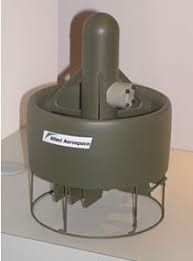
\includegraphics[scale=1]{Fig/iSTAR.jpg}
	\end{minipage}%
	\begin{minipage}[c]{0.5\textwidth}
		\centering
		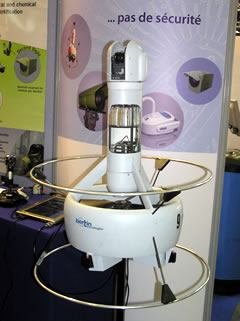
\includegraphics[scale=0.61]{Fig/Hovereye.png}
	\end{minipage}\\[1pt]
	\begin{minipage}[t]{.5\textwidth}
		\caption{\label{iSTAR}iSTAR}
	\end{minipage}%
	\begin{minipage}[t]{.5\textwidth}
		\caption{\label{Hovereye}Hovereye}
	\end{minipage}%
\end{figure}

由Bertin技术公司开发的Hoevereye用于搜集近距离的战斗情报,如图\ref{Hovereye}所示。其飞行续航时间为10分钟和航程达1.5公里。在32公里/小时的风速下,Hovereye的最大速度可以达到48公里/小时。Hoevereye具有不稳定的动力学特性,需要复杂的飞行控制系统才可以飞行\cite{Pflimlin_2006,Pflimlin_2007,Pflimlin_2007a,Pflimlin_2010}。
\begin{figure}[htbp]
	\centering
	\begin{minipage}[c]{0.5\textwidth}
		\centering
		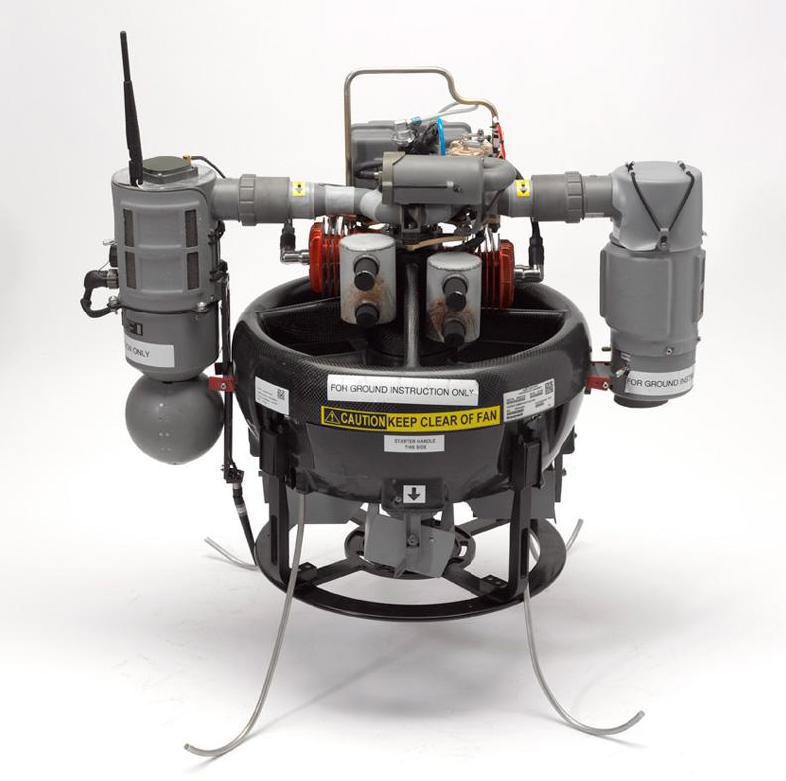
\includegraphics[width=6cm,height=6cm]{Fig/honeywell_t-hawk.jpg}
	\end{minipage}%
	\begin{minipage}[c]{0.5\textwidth}
		\centering
		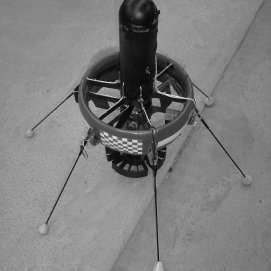
\includegraphics[width=6cm,height=6cm]{Fig/GTSpy.jpg}
	\end{minipage}\\[1pt]
	\begin{minipage}[t]{.5\textwidth}
		\caption{\label{Hawk}T-Hawk}
	\end{minipage}%
	\begin{minipage}[t]{.5\textwidth}
		\caption{\label{GTSpy}GTSpy}
	\end{minipage}%
\end{figure}

霍尼韦尔的T-Hawk因其曾被部署在真实的战场上而成名,如图\ref{Hawk}所示,它拥有两个小型汽油发动机。T-Hawk有40分钟的飞行续航力和在37公里/小时风速下最大速度90公里/小时。文献\parencite{Fleming_2004}介绍了T-Hawk RQ-16的空气动力学特性。

如图\ref{GTSpy}所示的是GTSpy,通过一个驱动双叶固定螺旋桨的油动发动机提供动力,六个控制舵位于涵道底部,最大重量为2.26公斤。GTSpy通过一种基于神经网络的自适应控制技术进行控制\cite{Johnson_2005}。

\begin{figure}[htbp]
	\centering
	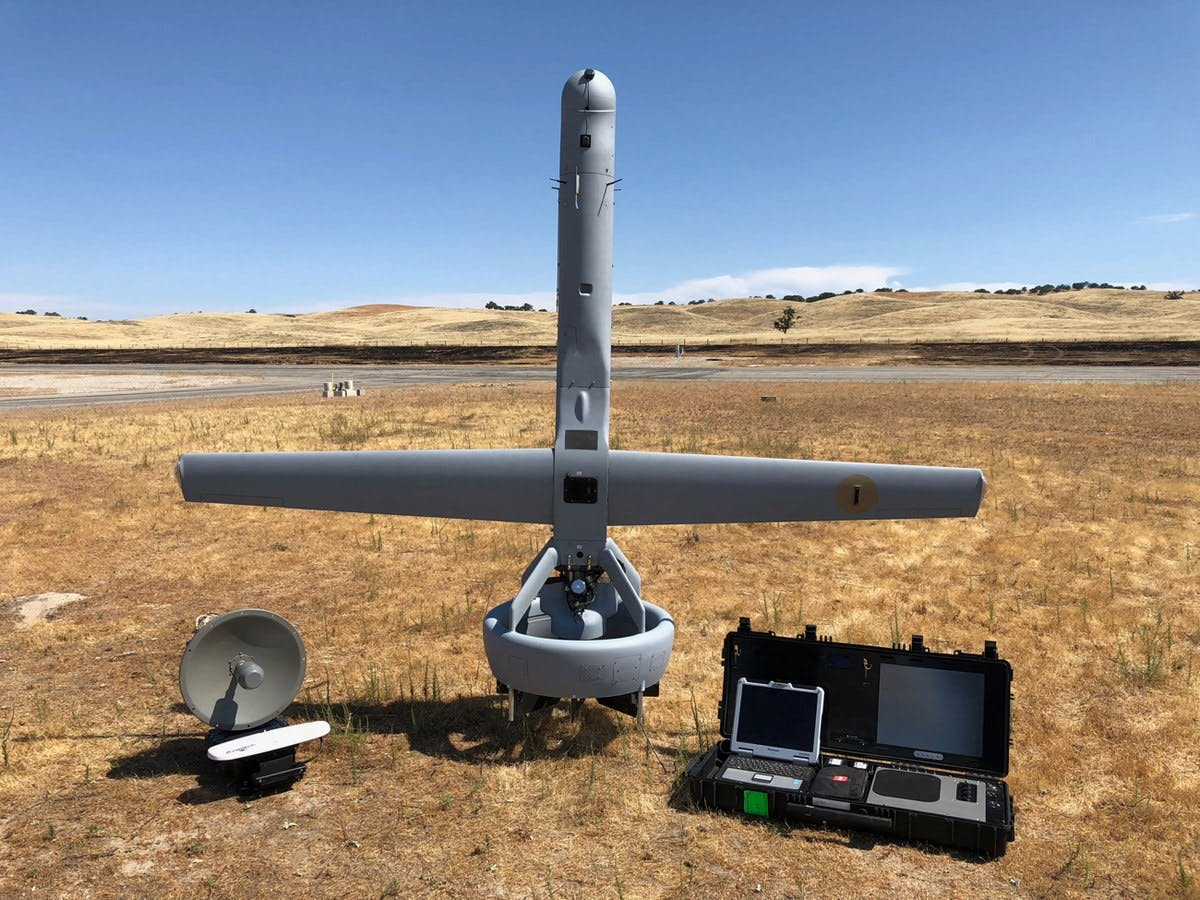
\includegraphics[width=6cm,height=4.5cm]{Fig/Fig_V-bat.jpeg}%
	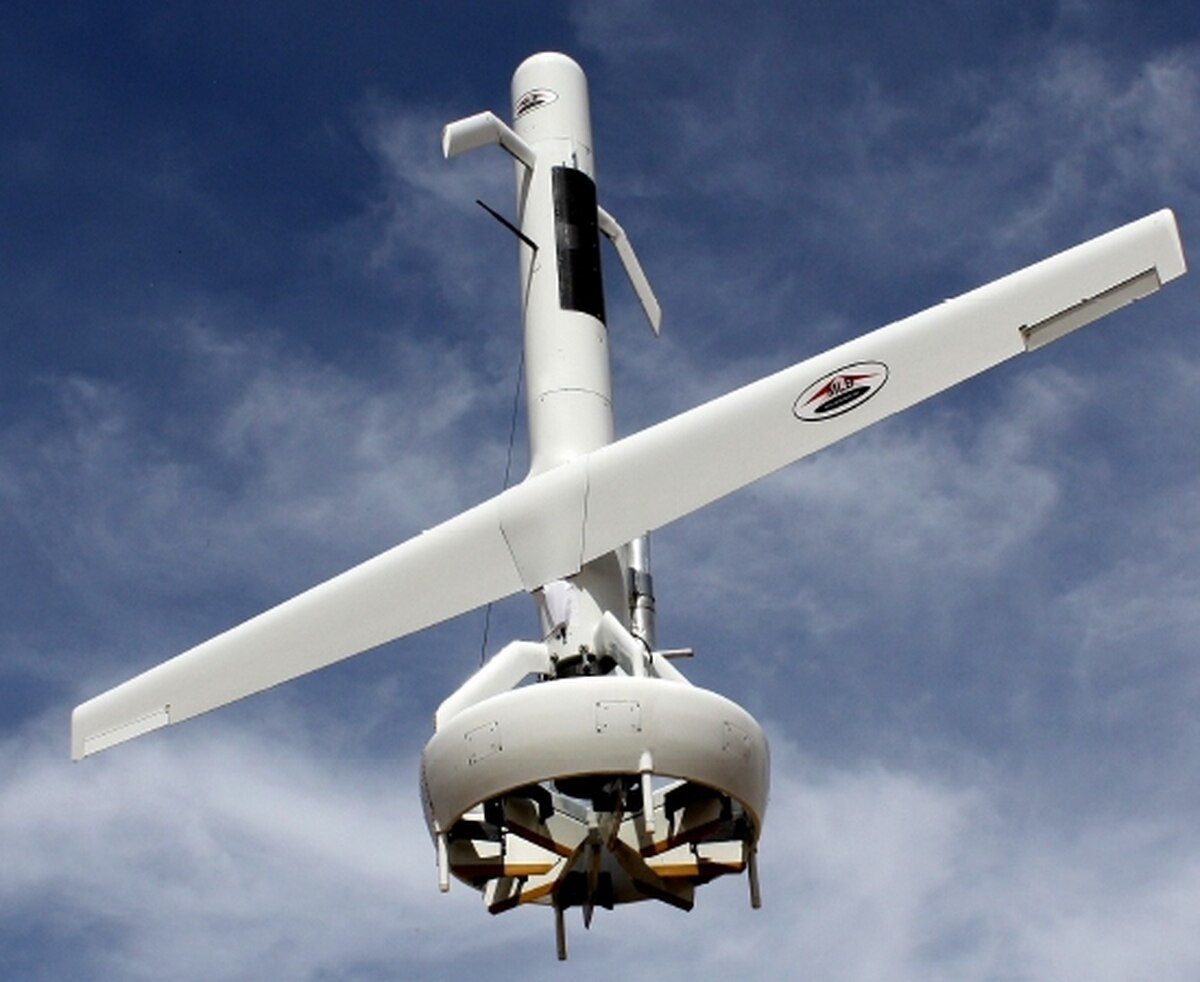
\includegraphics[width=6cm,height=4.5cm]{Fig/Fig_V-bat1.jpg}
	\caption{\label{Vbat}Vbat}
\end{figure}
图\ref{Vbat}是由美国Martin UAV公司开发的V-BAT\cite{Martin_},它可以从悬停过渡到固定机翼飞行模式并可以在没有俯冲下降的情况下再次切换回悬停模式。V-BAT可以完全自主地进行发射和回收,可在数分钟内打包和移动,在狭小的空间中操作非常方便。

相对单涵道而言,双涵道无人机的研究较少。利用双涵道飞行器也有着广阔的应用空间,如图\ref{Martin}所示的马丁背包(Martin  Jetpack),Martin Jetpack是一款小型VTOL设备,带有两个可提供升力的涵道风扇和一个汽油发动机。
\begin{figure}[htbp]
	\centering
	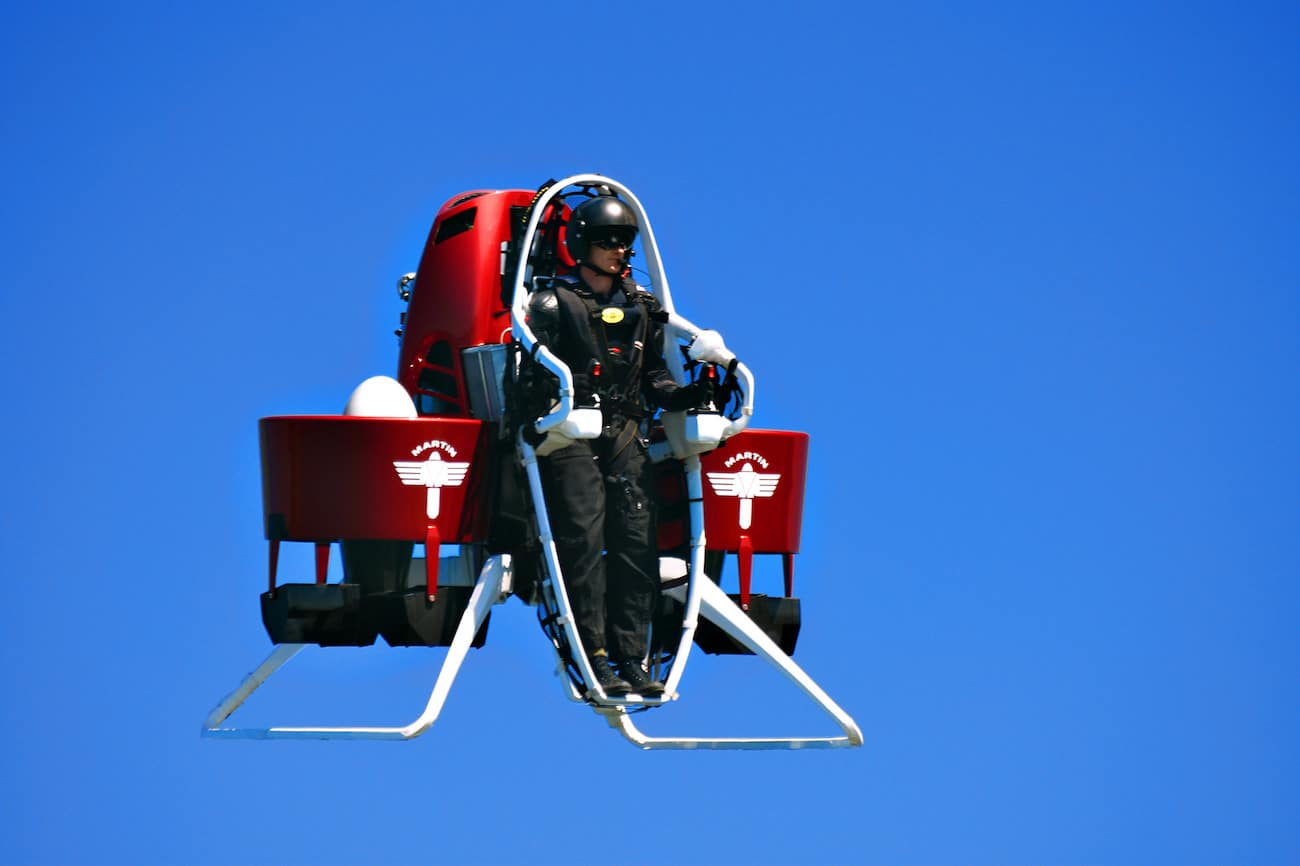
\includegraphics[width=10.4cm,height=6.928cm]{Fig/Martin-Jetpack-1.jpg}
	\caption{\label{Martin}Martin Jetpack}
\end{figure}

目前国内关于DFUAV的研究单/双涵道都有涉及,例如北京理工大学\cite{Wang_2018,Manzoor_2020},南京航空航天大学\cite{Zhao_2015},华南理工大学\cite{MengChaoHeng_}等。
\section{涵道风扇式无人机的控制方法研究现状}
%目前的控制器设计概述
精确的飞行器动力学模型对飞行控制系统至关重要。通常,旋转参数使用欧拉角或者四元数表示。大部分文献在建模时都将DFUAV视为刚体,使用牛顿-欧拉法建立动力学模型\cite{Choi_2011,Fleming_2003,Fleming_2004,Graf_2008,Johnson_2005,Ko_2007,Ohanian_2012,Pflimlin_2007a,Pflimlin_2010,Tobias_2008a,Zhao_2015,Zhengjie_2013}。

传统的PID控制应用较多。Pflimlin等人提出了基于PID的DFUAV姿态稳定策略\cite{Pflimlin_2007a}。文献\parencite{Manouchehri_2011}中使用一种基于PID控制器的悬停和前飞控制的双环控制策略。文献\parencite{Lipera_2001}采用PID控制器来实现iSTAR在悬停和低速飞行中的稳定性增强控制。Peddle等人介绍了将线性解耦估计器用作SLADe的反馈信号的连续闭环控制方法\cite{Peddle_2009}。文献\parencite{Pflimlin_2010}设计了一种PID控制器用于控制受测风影响的DFUAV的姿态。

现代控制方法也有应用。文献\parencite{Banazadeh_2014}将线性模型预测控制(LMPC)应用于DFUAV的控制中。Jeong等人将最优控制应用在DFUAV的飞行控制中\cite{Jeong_2015}。文献\parencite{Sharifzadeh_2019}在DFUAV的横向运动中上采用了NDI控制策略。文献\parencite{Marconi_2006}将非线性鲁棒控制应用到微型涵道无人机中,用于解决受参数不确定性影响的位置和姿态控制问题。

目前现代控制方法应用在DFUAV中大多停留在仿真阶段,实际应用中还是以PID控制为主。另一方面,DFUAV通常都冗余配置操纵面(超过三个),然而大多数和DFUAV控制有关的文献,都没有针对控制分配问题展开讨论。
\section{控制分配概述}
%目前DFUAV很少应用控制分配的研究成果,介绍这些成果
在飞行器、船舶等机械系统的运动控制中,操纵面是用于产生作用于系统的力或者力矩的机械装置,如推进器、舵、螺旋桨等。为了满足容错控制和控制重构等需求、提高系统的灵活性和动态响应,通常设计冗余的操纵面\cite{Johansen_2013}。DFUAV的操纵面是底部的气动舵面,气动舵面处于风扇滑流中,通过偏转舵面产生作用于涵道底部的侧向气动力来控制姿态。该类型无人机通常具有冗余的控制舵面,其姿态子系统是一个典型的过驱动(over-actuated)系统,因此在控制中存在控制分配问题。

操纵面冗余是设计过驱动系统的控制器时要解决的问题之一,一种常见的方法是设计最优控制构成闭环系统,操纵面指令即控制输入已经包含在设计中。另一种设计方法是引入伪控制输入(力或力矩)将调节或跟踪任务和控制分配任务分开,针对调节或跟踪任务设计的控制律作为伪控制输入的期望值,仅指定要产生的力或力矩,然后设计单独的控制分配模块,根据期望的力或力矩求解控制输入,文献\parencite{Harkegard_2005}讨论了两种设计方法的联系。这种分层设计的优点是可以单独设计控制律,而独立出来的控制分配模块不仅可以协调系统中不同操纵面的作用,还可以处理控制重构和操纵面容错之类的问题,例如文献\cite{Baggi_2020}利用控制分配对过驱动的小型固定翼无人机进行容错控制。本文的讨论是基于这种分层设计方法进行的,并将力矩或角加速度作为伪控制输入。

目前常用的控制分配方法包括伪逆法\cite{Golub_2012,Horn_2012}、直接分配法\cite{Durham_1993}、基于最优化方法的控制分配\cite{JohnA.M.Petersen_2005,Harkegard_2002}等,文献\parencite{Johansen_2013}对控制分配领域的成果做了详尽的调查。近年来,这些成果在航空\cite{Yan_2020}、航天\cite{Li_2018}、航海\cite{Garus_2017}、汽车\cite{Schwartz_2019}以及机器人\cite{Barthelmes_2017}等领域中得到广泛应用。然而,对于DFUAV的控制分配问题,大多数文献采用的求解方法都是伪逆法\cite{Pflimlin_2007a,Zhao_2015,Peddle_2009}。由于实际约束的存在,伪逆法无法对任意可达的期望力矩都返回容许控制\cite{Durham_2017},因此并不是最优的分配策略。

单涵道的控制分配问题的主要矛盾是可达集太小。在控制分配环节,由于存在约束,操纵面只能产生可达力矩集(Attainable Moment Set,AMS)内的力矩。控制律作为期望力矩,通常设计时已经考虑了AMS的范围,但某些情况下控制律仍可能会超出该范围。例如在飞行包络线的边界附近,操纵面无法产生控制律所要求的力矩,将存在分配误差,通常控制分配算法将返回一个在某种指标下误差最小的次最优解[3]。传统的控制分配算法返回次最优解时没有考虑控制律的分量的优先级问题,可能会使控制律的某些高优先级分量产生分配误差。由于DFUAV的特殊构型,在飞行中其期望力矩很可能超出AMS的范围。因此应用常规分配方法可能带来分配误差。

在双涵道控制分配中,操纵面的增加使得可达集也相应变大。分配问题的主要矛盾变为如何在不同带宽的执行器中分配伪控制输入,不可忽略的执行器动态带来了不良影响。
\section{本文的主要内容及章节安排}
控制分配与控制器设计、被控对象模型都有紧密的联系,本文的主题是研究涵道无人机的控制分配问题,而讨论控制分配问题不可避免要涉及建模以及控制器设计。因此本文将从以下几个方面展开:
\begin{enumerate}
	\item 	对一类涵道风扇式无人机——单涵道无人机和双涵道无人机,建立了非线性数学模型,并分析了其动力学特性。该部分的内容连同控制器、控制分配搭建的整个涵道无人机的飞行控制系统仿真,是本文的基础。目前单涵道的仿真已开源,代码下载地址:https://github.com/mengchaoheng/Plan-D。
	\item	如前文所述,DFUAV的气动特性复杂,再加上通道间有较强的耦合,其控制问题异常复杂。本文将自抗扰控制(ADRC)应用在DFUAV的姿态控制中,以提高系统抗干扰能力,降低扰动的影响。
	\item	所研究的DFUAV属于多操纵面飞行器,存在控制分配问题,本文将对基于ADRC进行姿态控制的一类DFUAV,讨论其控制分配问题。对于单涵道无人机,引入一种优先级分配方法。对于双涵道无人机,采用动态控制分配来解决双涵道无人机的控制分配问题。
	\item	对本文的核心内容进行仿真及飞行试验。	
\end{enumerate}

根据以上内容,本文的章节安排如下:

第一章,绪论。本章首先介绍了本文的研究背景及意义,回顾了DFUAV的发展现状以及控制方法、控制分配方法的研究现状及其在DFUAV中的应用。

第二章,涵道风扇式无人机建模。在这一章章中,我们首先应用牛顿-欧拉法推导了DFUAV的运动方程,然后分别对单涵道和双涵道的分析了作用于机体的气动力以及气动力矩。最后根据被控对象数学模型搭建了无人机六自由度运动Simulink$^\circledR$仿真模型。

第三章,自抗扰控制器设计。本章引入ADRC控制方法用于DFUAV的姿态控制。首先介绍了ADRCD各组成部分的基本原理,接着不加证明地给出收敛性分析。然后设计ADRC控制器并说明其满足收敛性条件。最后将所设计的控制器实现到MATLAB$^\circledR$/Simulink$^\circledR$中。

第四章,涵道风扇式无人机的控制分配。本章分别对单涵道和双涵道的控制分配问题进行了分析,根据各自的特点,分别使用不同的方法求解。
%对于单涵道,指出目前广泛应用的伪逆法的不足,并分析了单涵道控制分配主要的难题是可达集太小。我们根据自抗扰控制律中各组成部分优先级不同这一事实,提出优先级分配方法。在推导优先级分配法时,借助了直接分配法的思路,推导了任意有限个优先级排序的伪控制指令的分配问题。对于双涵道,针对操纵面中包含不同动态特性的执行器且其动力学不可忽略的问题,借助动态控制分配进行求解。

第五章,仿真及飞行试验。本章包含仿真和飞行试验两部分。在单涵道仿真中,首先通过相同输入、相同控制器下对比真实飞行数据和仿真输出,佐证了建模的准确度。再将仿真模型用于验证所设计的ADRC控制器的有效性。接着考察优先级分配法对伪控制输入的跟踪。在双涵道仿真中,仅针对伪控制输入的分配情况进行分析。飞行试验部分,将ADRC控制以及优先级控制分配应用到单涵道中进行飞行试验,考察了优先级方法的输出解耦能力以及扰动抑制效果。

第六章,总结。本章给出了本文的主要结论,指明了本文的创新点以及不足之处,并指出今后进一步在飞行器控制分配领域进行研究工作的展望与设想。

